\documentclass[12pt, openany, letterpaper]{memoir}
\usepackage{HomeworkStyle}

\begin{document}

\begin{center}
	{\large Homework 5 -- Simple Mixtures}
\end{center}

Name: \rule[-.1mm]{15em}{0.1pt}

\begin{description}
	\item [Exercise 5A.9(a)] ~ (5 points)

	      At $300~K$, the partial vapor pressure of \ch{HCl} (that is, the partial pressure of the \ch{HCl} vapor) in liquid \ch{GeCl4} is as follows:

	      \begin{tabular}{c|c|c|c}
		      $\chi_{\ch{HCl}}$   & $0.005$ & $0.012$ & $0.019$ \\
		      $p_{\ch{HCl}}(kPa)$ & $32.0$  & $76.9$  & $121.8$
	      \end{tabular}

	      Show that the solution obeys Henry's law in this range of mole fractions, and calculate the Henry's law constant at $300~K$

	      \vspace{15em}
	\item [Exercise 5B.2(a)] ~ (5 points)
	      The vapor pressure of benzene is $53.3~kPa$ at $60.6^\circ C$, but it fell to $51.5~kPa$ when $19.0~g$ of a non-volatile organic copound was dissolved in $500~g$ of benzene. Calculate the molar mass of the compound


	      \vspace{20em}
	\item [My Problem 1] ~ (10 points)

	      Below are the bubble-point and dew-point curves (liquid/vapor composition curves) for a mixture of hexane in heptane. Consider a mixture of $10.0~g$ of hexane in $10.0~g$ of heptane at $T=85^\circ C$. Find the following for this mixture: $\circled{1}$ The compositions of the liquid and vapor phases, and $\circled{2}$ the fraction of molecules in the liquid phase. Note that the curves have been fit to cubic functions, which allows for precise answers.

	      \noindent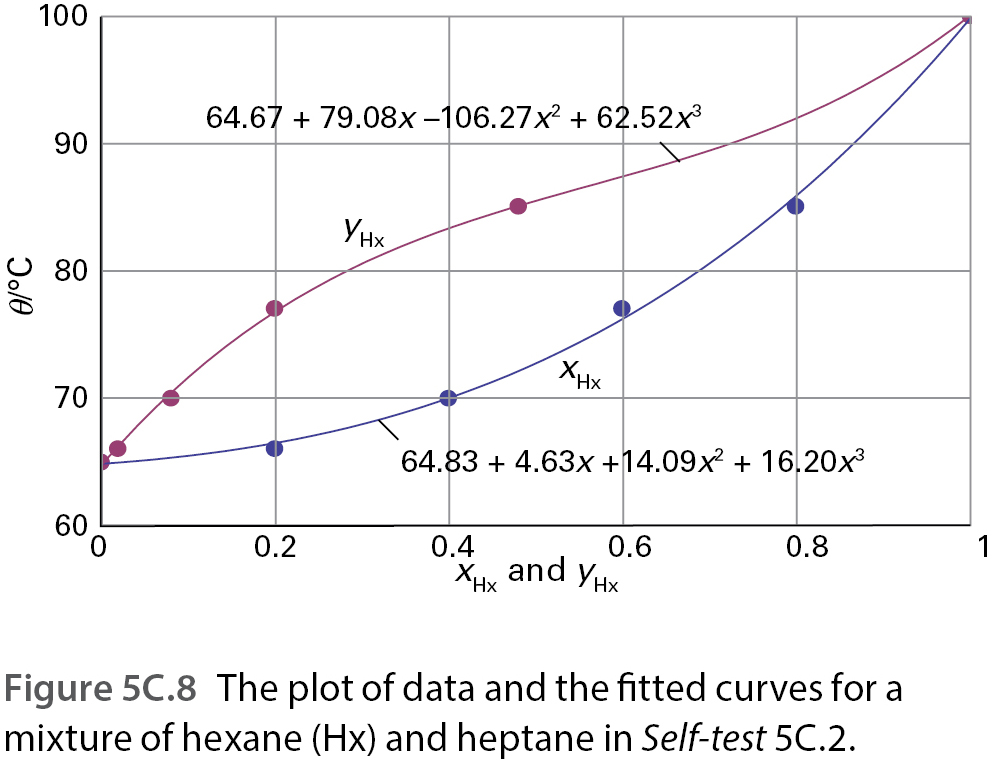
\includegraphics[width=0.5\linewidth]{Mixture_Curve}

	      \vspace{35em}
	\item [My Problem 2] ~ (5 points)

	      Below are the composition curves for a certain azeotrope. Suppose you have a sample of this mixture with composition $Z_A = a$ (the dashed line marked $a$). In the limit of a many-stage distillation carried out until compositions are stable, what will be the compositions of the liquid and vapor phases?

	      \noindent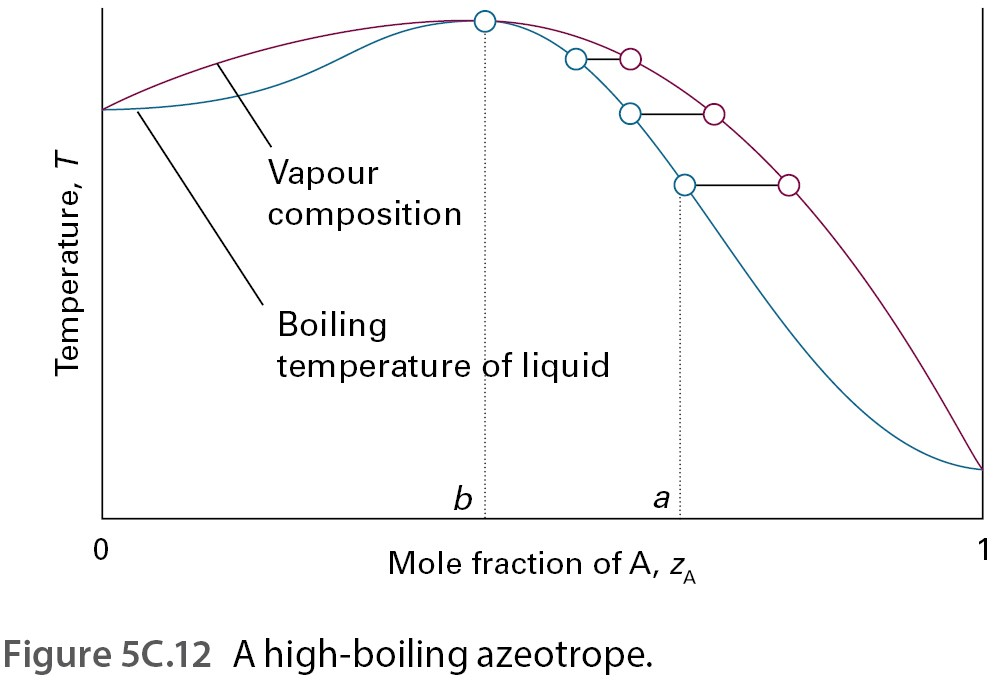
\includegraphics[width=0.5\linewidth]{Azeotrope}

	\item [My Problem 3] ~ (10 points)

	      Below are the composition curves for a mixture near its freezing point. The eutectic composition ($e_2$ in the figure) is at $\chi_B = 0.42$. Suppose you have a liquid with $3.0~moles$ of $B$ and $1.0~mole$ of $A$. This mixture has $\chi_B=0.75$ ($a$ in the figure), and is cooled slowly until it just reaches the eutectic freezing point. Find the following at this point: $\circled{1}$ The compositions of the solid and liquid phases, and $\circled{2}$ the number of moles in the solid phase.

	      \noindent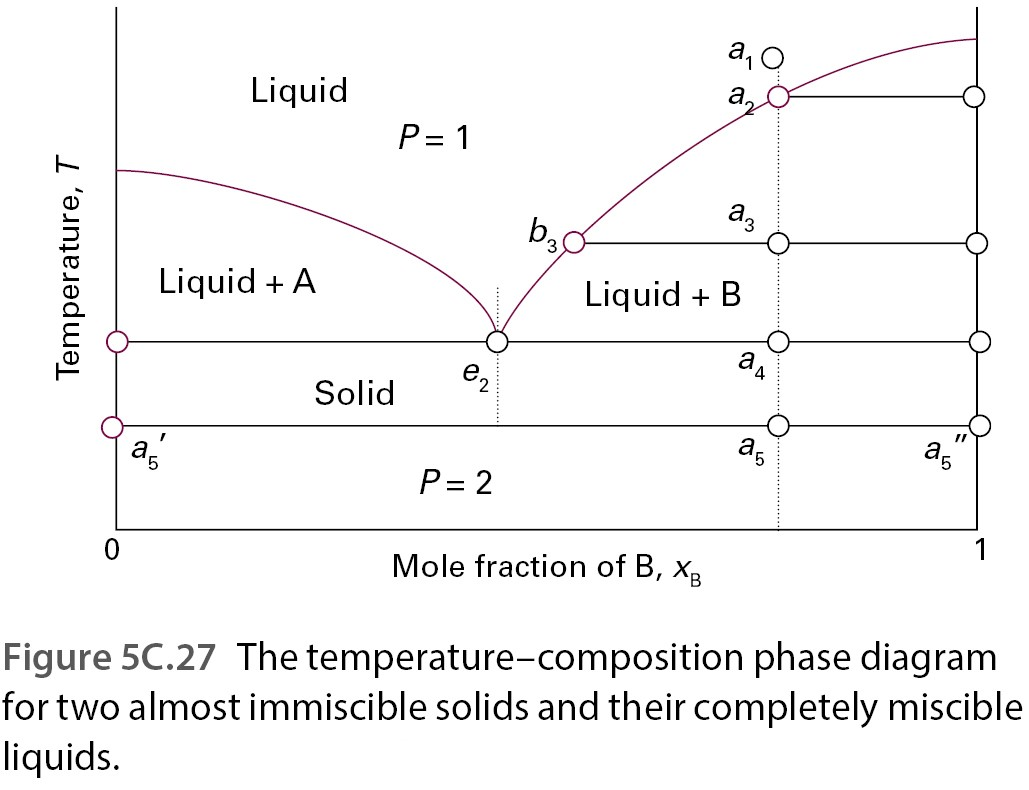
\includegraphics[width=0.5\linewidth]{Eutectic}
	      \vspace{15em}

	\item [Exercise 5F.3(a)] ~ (5 points)

	      Estimate the mean ionic activity coefficient ($\gamma_\pm$) and activity of a solution at $25^\circ C$ that is $0.010~\nicefrac{mol}{kg}$ \ch{CaCl2(aq)} and $0.030~\nicefrac{mol}{kg}$ \ch{NaF(aq)}.

	      \vspace{18em}
	\item [My Problem 4] ~ (10 points)

	      \ch{CaF2} is a sparingly soluble salt whose solubility product is $K_{SP}=1.6\times10^{-10}$. Give the molar concentration of \ch{CaF2} in $\circled{1}$ pure water, and $\circled{2}$ an aqueous solution buffered with $0.50~molal$ \ch{NaNO3}. Use the extended Debye-H\"uckel law, with $A=0.5085$ and $B=0.9843$ (values for water at $25^\circ C$ and typical ion sizes).

\end{description}

\newpage
\pagestyle{empty}
\addtocounter{page}{-1}
\section*{\emph{Slaveships}}
\paragraph{By Lucille Clifton}~
\begin{verse}
	loaded like spoons\\
	into the belly of Jesus\\
	where we lay for weeks for months\\
	in the sweat and stink\\
	of our own breathing\\
	Jesus\\
	why do you not protect us\\
	chained to the heart of the Angel\\
	where the prayers we never tell\\
	and hot and red\\
	as our bloody ankles\\
	Jesus\\
	Angel\\
	can these be men\\
	who vomit us out from ships\\
	called Jesus    Angel    Grace of God\\
	onto a heathen country\\
	Jesus\\
	Angel\\
	ever again\\
	can this tongue speak\\
	can these bones walk\\
	Grace Of God\\
	can this sin live
\end{verse}
\end{document}
